%%*************************************************************************
%% Legal Notice:
%% This code is offered as-is without any warranty either expressed or
%% implied; without even the implied warranty of MERCHANTABILITY or
%% FITNESS FOR A PARTICULAR PURPOSE! 
%% User assumes all risk.
%% In no event shall IEEE or any contributor to this code be liable for
%% any damages or losses, including, but not limited to, incidental,
%% consequential, or any other damages, resulting from the use or misuse
%% of any information contained here.
%%
%% All comments are the opinions of their respective authors and are not
%% necessarily endorsed by the IEEE.
%%
%% This work is distributed under the LaTeX Project Public License (LPPL)
%% ( http://www.latex-project.org/ ) version 1.3, and may be freely used,
%% distributed and modified. A copy of the LPPL, version 1.3, is included
%% in the base LaTeX documentation of all distributions of LaTeX released
%% 2003/12/01 or later.
%% Retain all contribution notices and credits.
%% ** Modified files should be clearly indicated as such, including  **
%% ** renaming them and changing author support contact information. **
%%
%% File list of work: IEEEtran.cls, IEEEtran_HOWTO.pdf, bare_adv.tex,
%%                    bare_conf.tex, bare_jrnl.tex, bare_jrnl_compsoc.tex
%%*************************************************************************

% *** Authors should verify (and, if needed, correct) their LaTeX system  ***
% *** with the testflow diagnostic prior to trusting their LaTeX platform ***
% *** with production work. IEEE's font choices can trigger bugs that do  ***
% *** not appear when using other class files.                            ***
% The testflow support page is at:
% http://www.michaelshell.org/tex/testflow/



% Note that the a4paper option is mainly intended so that authors in
% countries using A4 can easily print to A4 and see how their papers will
% look in print - the typesetting of the document will not typically be
% affected with changes in paper size (but the bottom and side margins will).
% Use the testflow package mentioned above to verify correct handling of
% both paper sizes by the user's LaTeX system.
%
% Also note that the "draftcls" or "draftclsnofoot", not "draft", option
% should be used if it is desired that the figures are to be displayed in
% draft mode.
%
\documentclass[conference]{IEEEtran}
% Add the compsoc option for Computer Society conferences.
%
% If IEEEtran.cls has not been installed into the LaTeX system files,
% manually specify the path to it like:
% \documentclass[conference]{../sty/IEEEtran}





% Some very useful LaTeX packages include:
% (uncomment the ones you want to load)


% *** MISC UTILITY PACKAGES ***
%
%\usepackage{ifpdf}
% Heiko Oberdiek's ifpdf.sty is very useful if you need conditional
% compilation based on whether the output is pdf or dvi.
% usage:
% \ifpdf
%   % pdf code
% \else
%   % dvi code
% \fi
% The latest version of ifpdf.sty can be obtained from:
% http://www.ctan.org/tex-archive/macros/latex/contrib/oberdiek/
% Also, note that IEEEtran.cls V1.7 and later provides a builtin
% \ifCLASSINFOpdf conditional that works the same way.
% When switching from latex to pdflatex and vice-versa, the compiler may
% have to be run twice to clear warning/error messages.






% *** CITATION PACKAGES ***
%
%\usepackage{cite}
% cite.sty was written by Donald Arseneau
% V1.6 and later of IEEEtran pre-defines the format of the cite.sty package
% \cite{} output to follow that of IEEE. Loading the cite package will
% result in citation numbers being automatically sorted and properly
% "compressed/ranged". e.g., [1], [9], [2], [7], [5], [6] without using
% cite.sty will become [1], [2], [5]--[7], [9] using cite.sty. cite.sty's
% \cite will automatically add leading space, if needed. Use cite.sty's
% noadjust option (cite.sty V3.8 and later) if you want to turn this off.
% cite.sty is already installed on most LaTeX systems. Be sure and use
% version 4.0 (2003-05-27) and later if using hyperref.sty. cite.sty does
% not currently provide for hyperlinked citations.
% The latest version can be obtained at:
% http://www.ctan.org/tex-archive/macros/latex/contrib/cite/
% The documentation is contained in the cite.sty file itself.






% *** GRAPHICS RELATED PACKAGES ***
%
\ifCLASSINFOpdf
\usepackage[pdftex]{graphicx}
  % declare the path(s) where your graphic files are
\graphicspath{{./images/}}
  % and their extensions so you won't have to specify these with
  % every instance of \includegraphics
\DeclareGraphicsExtensions{.jpg,.png}
\else
  % or other class option (dvipsone, dvipdf, if not using dvips). graphicx
  % will default to the driver specified in the system graphics.cfg if no
  % driver is specified.
  % \usepackage[dvips]{graphicx}
  % declare the path(s) where your graphic files are
  % \graphicspath{{../eps/}}
  % and their extensions so you won't have to specify these with
  % every instance of \includegraphics
  % \DeclareGraphicsExtensions{.eps}
\fi
% graphicx was written by David Carlisle and Sebastian Rahtz. It is
% required if you want graphics, photos, etc. graphicx.sty is already
% installed on most LaTeX systems. The latest version and documentation can
% be obtained at: 
% http://www.ctan.org/tex-archive/macros/latex/required/graphics/
% Another good source of documentation is "Using Imported Graphics in
% LaTeX2e" by Keith Reckdahl which can be found as epslatex.ps or
% epslatex.pdf at: http://www.ctan.org/tex-archive/info/
%
% latex, and pdflatex in dvi mode, support graphics in encapsulated
% postscript (.eps) format. pdflatex in pdf mode supports graphics
% in .pdf, .jpeg, .png and .mps (metapost) formats. Users should ensure
% that all non-photo figures use a vector format (.eps, .pdf, .mps) and
% not a bitmapped formats (.jpeg, .png). IEEE frowns on bitmapped formats
% which can result in "jaggedy"/blurry rendering of lines and letters as
% well as large increases in file sizes.
%
% You can find documentation about the pdfTeX application at:
% http://www.tug.org/applications/pdftex





% *** MATH PACKAGES ***
%
%\usepackage[cmex10]{amsmath}
% A popular package from the American Mathematical Society that provides
% many useful and powerful commands for dealing with mathematics. If using
% it, be sure to load this package with the cmex10 option to ensure that
% only type 1 fonts will utilized at all point sizes. Without this option,
% it is possible that some math symbols, particularly those within
% footnotes, will be rendered in bitmap form which will result in a
% document that can not be IEEE Xplore compliant!
%
% Also, note that the amsmath package sets \interdisplaylinepenalty to 10000
% thus preventing page breaks from occurring within multiline equations. Use:
%\interdisplaylinepenalty=2500
% after loading amsmath to restore such page breaks as IEEEtran.cls normally
% does. amsmath.sty is already installed on most LaTeX systems. The latest
% version and documentation can be obtained at:
% http://www.ctan.org/tex-archive/macros/latex/required/amslatex/math/





% *** SPECIALIZED LIST PACKAGES ***
%
%\usepackage{algorithmic}
% algorithmic.sty was written by Peter Williams and Rogerio Brito.
% This package provides an algorithmic environment fo describing algorithms.
% You can use the algorithmic environment in-text or within a figure
% environment to provide for a floating algorithm. Do NOT use the algorithm
% floating environment provided by algorithm.sty (by the same authors) or
% algorithm2e.sty (by Christophe Fiorio) as IEEE does not use dedicated
% algorithm float types and packages that provide these will not provide
% correct IEEE style captions. The latest version and documentation of
% algorithmic.sty can be obtained at:
% http://www.ctan.org/tex-archive/macros/latex/contrib/algorithms/
% There is also a support site at:
% http://algorithms.berlios.de/index.html
% Also of interest may be the (relatively newer and more customizable)
% algorithmicx.sty package by Szasz Janos:
% http://www.ctan.org/tex-archive/macros/latex/contrib/algorithmicx/




% *** ALIGNMENT PACKAGES ***
%
%\usepackage{array}
% Frank Mittelbach's and David Carlisle's array.sty patches and improves
% the standard LaTeX2e array and tabular environments to provide better
% appearance and additional user controls. As the default LaTeX2e table
% generation code is lacking to the point of almost being broken with
% respect to the quality of the end results, all users are strongly
% advised to use an enhanced (at the very least that provided by array.sty)
% set of table tools. array.sty is already installed on most systems. The
% latest version and documentation can be obtained at:
% http://www.ctan.org/tex-archive/macros/latex/required/tools/


%\usepackage{mdwmath}
%\usepackage{mdwtab}
% Also highly recommended is Mark Wooding's extremely powerful MDW tools,
% especially mdwmath.sty and mdwtab.sty which are used to format equations
% and tables, respectively. The MDWtools set is already installed on most
% LaTeX systems. The lastest version and documentation is available at:
% http://www.ctan.org/tex-archive/macros/latex/contrib/mdwtools/


% IEEEtran contains the IEEEeqnarray family of commands that can be used to
% generate multiline equations as well as matrices, tables, etc., of high
% quality.


%\usepackage{eqparbox}
% Also of notable interest is Scott Pakin's eqparbox package for creating
% (automatically sized) equal width boxes - aka "natural width parboxes".
% Available at:
% http://www.ctan.org/tex-archive/macros/latex/contrib/eqparbox/





% *** SUBFIGURE PACKAGES ***
%\usepackage[tight,footnotesize]{subfigure}
% subfigure.sty was written by Steven Douglas Cochran. This package makes it
% easy to put subfigures in your figures. e.g., "Figure 1a and 1b". For IEEE
% work, it is a good idea to load it with the tight package option to reduce
% the amount of white space around the subfigures. subfigure.sty is already
% installed on most LaTeX systems. The latest version and documentation can
% be obtained at:
% http://www.ctan.org/tex-archive/obsolete/macros/latex/contrib/subfigure/
% subfigure.sty has been superceeded by subfig.sty.



%\usepackage[caption=false]{caption}
%\usepackage[font=footnotesize]{subfig}
% subfig.sty, also written by Steven Douglas Cochran, is the modern
% replacement for subfigure.sty. However, subfig.sty requires and
% automatically loads Axel Sommerfeldt's caption.sty which will override
% IEEEtran.cls handling of captions and this will result in nonIEEE style
% figure/table captions. To prevent this problem, be sure and preload
% caption.sty with its "caption=false" package option. This is will preserve
% IEEEtran.cls handing of captions. Version 1.3 (2005/06/28) and later 
% (recommended due to many improvements over 1.2) of subfig.sty supports
% the caption=false option directly:
%\usepackage[caption=false,font=footnotesize]{subfig}
%
% The latest version and documentation can be obtained at:
% http://www.ctan.org/tex-archive/macros/latex/contrib/subfig/
% The latest version and documentation of caption.sty can be obtained at:
% http://www.ctan.org/tex-archive/macros/latex/contrib/caption/




% *** FLOAT PACKAGES ***
%
%\usepackage{fixltx2e}
% fixltx2e, the successor to the earlier fix2col.sty, was written by
% Frank Mittelbach and David Carlisle. This package corrects a few problems
% in the LaTeX2e kernel, the most notable of which is that in current
% LaTeX2e releases, the ordering of single and double column floats is not
% guaranteed to be preserved. Thus, an unpatched LaTeX2e can allow a
% single column figure to be placed prior to an earlier double column
% figure. The latest version and documentation can be found at:
% http://www.ctan.org/tex-archive/macros/latex/base/



\usepackage{stfloats}
% stfloats.sty was written by Sigitas Tolusis. This package gives LaTeX2e
% the ability to do double column floats at the bottom of the page as well
% as the top. (e.g., "\begin{figure*}[!b]" is not normally possible in
% LaTeX2e). It also provides a command:
%\fnbelowfloat
% to enable the placement of footnotes below bottom floats (the standard
% LaTeX2e kernel puts them above bottom floats). This is an invasive package
% which rewrites many portions of the LaTeX2e float routines. It may not work
% with other packages that modify the LaTeX2e float routines. The latest
% version and documentation can be obtained at:
% http://www.ctan.org/tex-archive/macros/latex/contrib/sttools/
% Documentation is contained in the stfloats.sty comments as well as in the
% presfull.pdf file. Do not use the stfloats baselinefloat ability as IEEE
% does not allow \baselineskip to stretch. Authors submitting work to the
% IEEE should note that IEEE rarely uses double column equations and
% that authors should try to avoid such use. Do not be tempted to use the
% cuted.sty or midfloat.sty packages (also by Sigitas Tolusis) as IEEE does
% not format its papers in such ways.





% *** PDF, URL AND HYPERLINK PACKAGES ***
%
%\usepackage{url}
% url.sty was written by Donald Arseneau. It provides better support for
% handling and breaking URLs. url.sty is already installed on most LaTeX
% systems. The latest version can be obtained at:
% http://www.ctan.org/tex-archive/macros/latex/contrib/misc/
% Read the url.sty source comments for usage information. Basically,
% \url{my_url_here}.





% *** Do not adjust lengths that control margins, column widths, etc. ***
% *** Do not use packages that alter fonts (such as pslatex).         ***
% There should be no need to do such things with IEEEtran.cls V1.6 and later.
% (Unless specifically asked to do so by the journal or conference you plan
% to submit to, of course. )


% correct bad hyphenation here
\hyphenation{op-tical net-works semi-conduc-tor}


\begin{document}
%
% paper title
% can use linebreaks \\ within to get better formatting as desired
\title{Integrating Droplet into Applab -- Improving The Usability of a Blocks-Based Text Editor}


% author names and affiliations
% use a multiple column layout for up to three different
% affiliations
\author{\IEEEauthorblockN{David Anthony Bau}
\IEEEauthorblockA{Phillips Exeter Academy\\
Exeter, New Hampshire 03833\\
Email: dbau@exeter.edu}
}

% conference papers do not typically use \thanks and this command
% is locked out in conference mode. If really needed, such as for
% the acknowledgment of grants, issue a \IEEEoverridecommandlockouts
% after \documentclass

% for over three affiliations, or if they all won't fit within the width
% of the page, use this alternative format:
% 
%\author{\IEEEauthorblockN{Michael Shell\IEEEauthorrefmark{1},
%Homer Simpson\IEEEauthorrefmark{2},
%James Kirk\IEEEauthorrefmark{3}, 
%Montgomery Scott\IEEEauthorrefmark{3} and
%Eldon Tyrell\IEEEauthorrefmark{4}}
%\IEEEauthorblockA{\IEEEauthorrefmark{1}School of Electrical and Computer Engineering\\
%Georgia Institute of Technology,
%Atlanta, Georgia 30332--0250\\ Email: see http://www.michaelshell.org/contact.html}
%\IEEEauthorblockA{\IEEEauthorrefmark{2}Twentieth Century Fox, Springfield, USA\\
%Email: homer@thesimpsons.com}
%\IEEEauthorblockA{\IEEEauthorrefmark{3}Starfleet Academy, San Francisco, California 96678-2391\\
%Telephone: (800) 555--1212, Fax: (888) 555--1212}
%\IEEEauthorblockA{\IEEEauthorrefmark{4}Tyrell Inc., 123 Replicant Street, Los Angeles, California 90210--4321}}




% use for special paper notices
%\IEEEspecialpapernotice{(Invited Paper)}




% make the title area
\maketitle


\begin{abstract}
%\boldmath
Droplet is a new programming editor that allows dual-mode editing in blocks and text for any text program. This paper presents observations and improvements to Droplet based on integrating Droplet into Applab, Code.org's JavaScript sandbox learning environment. Droplet's unique interactions with both text and blocks create several unusual problems and opportunities for improvement.

\end{abstract}
% IEEEtran.cls defaults to using nonbold math in the Abstract.
% This preserves the distinction between vectors and scalars. However,
% if the conference you are submitting to favors bold math in the abstract,
% then you can use LaTeX's standard command \boldmath at the very start
% of the abstract to achieve this. Many IEEE journals/conferences frown on
% math in the abstract anyway.

% no keywords




% For peer review papers, you can put extra information on the cover
% page as needed:
% \ifCLASSOPTIONpeerreview
% \begin{center} \bfseries EDICS Category: 3-BBND \end{center}
% \fi
%
% For peerreview papers, this IEEEtran command inserts a page break and
% creates the second title. It will be ignored for other modes.
\IEEEpeerreviewmaketitle

\section{Introduction}
  This paper describes the development of a series of usability improvements for a Droplet block editor. Droplet provides a visual editing mode similar to Scratch \cite{Scratch}, Alice \cite{Alice}, and Blockly \cite{Blockly}. However, Droplet is unique because it works as a text editor, and provides a block interface on top of parsed text code. Initially, Droplet provided the following features:

\begin{itemize}
  \item Blocks based on parsed text allowing lossless conversion between blocks and text.
  \item A palette of short prewritten code fragments, represented as blocks.
  \item An editor supporting drag-and-drop assembly and editing of the blocks in a linear program.
\end{itemize}

  Because Droplet is a text editor, many features of other block languages were initially implemented. For example, Weintrop \cite{Weintrop} found that a key benefit of block languages is that the two-dimensional surface allows bottom-up assembly of code. However, because of the linear nature of text code, the first version of Droplet did not support it.

  In this work, the goal of the author has been to carefully consider usability principles in the context of block editors, and to find ways to implement important usability improvements in Droplet.

  The principles we recognized and considered were:

\begin{enumerate}
  \item Two dimensional code assembly, as proposed by Weintrop \cite{Weintrop}. The challenge is to relate this to the underlying linear text code.
  \item User control and freedom through undo. In the context of block editing, two forms of undo are important.  Both were implemented and are described here.
  \item Recognition versus recall.  Although the block palette is an aid for remembering commands, an aid is needed for remembering text socket values, in a way that is compatible with text coding.
  \item Error messages and warnings. Droplet can edit any text program and therefore can create programs with errors. To help users with errors, it is helpful to borrow ideas from traditional text programming editors.
\end{enumerate}

  In this paper the author describes solutions for these four usability issues. The work was done in the context of integrating Droplet's Javascript mode into Code.org's Applab environment. This paper also compares Droplet's approach to the approaches taken by Scratch and Blockly.
\section{Background}
\begin{figure*}
\centering
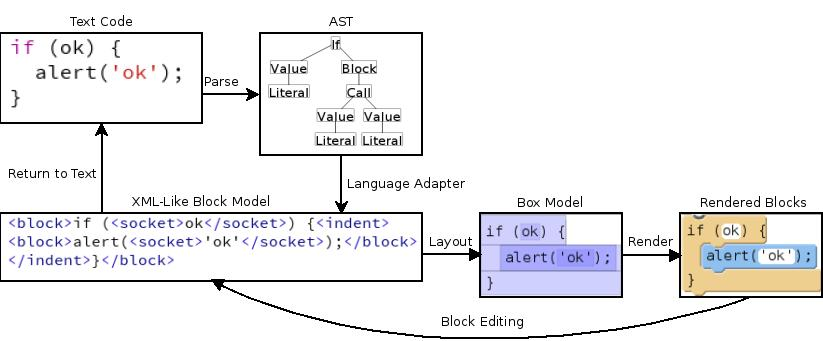
\includegraphics[width=5in]{lifecycle.jpg}
\caption{Droplet's Lifecycle for a JavaScript Program}
\label{lifecycle}
\end{figure*}

Droplet is an editor that display text code as visual blocks, and can toggle between the two. A Droplet document is simply a text file which Droplet annotates with markup for editing purposes. Figure \ref{lifecycle} shows the lifecycle of a Droplet program in JavaScript. When the user opens a file, the language adapter for JavaScript is invoked and runs the code through a standard JavaScript parser. It uses the resulting syntax tree to annotate the text stream with tokens like "blockStart" or "socketEnd" to indicate where block entities should be rendered. The adapter also attaches metadata to the blocks about color, shape, and droppability rules. Droplet then lays out and renders the resulting stream. When the user saves or runs the file, the markup is simply discarded and, if no edits have occurred, the original text stream is guaranteed to be generated again.

Droplet's layout algorithm always places text nodes in the same rows as the text appeared in the source. This allows Droplet to achieve a smooth animation between blocks and text.

\section{Relating Floating Stacks to Text Code}

A study by Weintrop \cite{Weintrop} found that Scratch's two-dimensional editing surface was beneficial to students. It allowed students to try out different ways of performing the same task, and to compose programs in a "non-linear" way. Maloney et al. \cite{Maloney} refer to this as "tinkerability," and say that it supports "a bottom-up approach to writing scripts where small chunks of code are assembled and tested, then combined into larger units." This layout, however, is unfriendly to the linear nature of text code. Droplet needed a way to support assembling and viewing code side-by-side while retaining a one-to-one relationship to text code.

Both Scratch and Blockly support floating blocks. Blockly runs all floating code in top-left to bottom-right order, while each Scratch block stack is associated with an event handler and runs whenever the attached event is fired. Scratch also runs a stack when it is double-clicked.

\begin{figure}
\centering
\includegraphics[width=2.5in]{floating-blocks.png}
\caption{An Example of Droplet's Floating Block Graphics}
\label{floating}
\end{figure}

Droplet now allows floating blocks to be assembled, but surrounds them with a dotted line and the language's block comment symbol to indicate that they are not going to be run (fig. \ref{floating}). The surrounding dotted line can be grabbed to move the entire stack or replace it into the main document to "uncomment" it. This allows students to assemble blocks in a nonlinear order, and borrows metaphors from text to make it clear that the stacks will not be run. Dropet can also display a "play" button (as seen in figure \ref{floating}) and emit an event to support running individual stacks.

In the future, Droplet may represent these blocks in the code by inserting them as comments. This would allow Droplet show an animation between the floating stacks in text mode and in block mode.

\section{User Control and Freedom}

Especially in untyped languages like JavaScript, it is easy to accidentally drop Droplet blocks into the wrong socket. However, because Droplet is text-based, sockets often contain important information like long strings. Other major block languages do not have this problem because sockets with information like variable names or strings are not usually drop targets for other blocks.

Blockly does not have this problem, because most constants that could be long, sensitive work are not also drop targets for other blocks. In Blockly, typing socket, which is round, is different from a droppable socket, which looks like a puzzle piece, so work is not lost when an accidental drop occurs.

Scratch has this problem, but it is less pronounced, since sockets that contain strings are not drop targets. Scratch repopulates sockets with hand-chosen default values when blocks are dragged out of them.

Neither Scratch nor Blockly implements a full undo stack. Blockly has progress on an undo stack based on the serialized operations it will make for real-time collaboration. Scratch does not have an undo stack, but has support for "undeleting" the last block that was deleted.

\subsection{Full Support for Undo and Redo}
Undo stacks are important to usability, and are included in Neilsen's widely-recognized user interface heuristics \cite{Neilsen}. Undo was difficult to implement in Droplet because of the way Droplet reparses and replaces blocks whenever they are changed, invalidating pointers to blocks. Droplet needed a clean model for serializing and maintaining the locations of blocks in the document.

Droplet now supports two different locations models: a token-based locations model identifying blocks by their token offset from the beginning of the document, and a text-based locations model identifying blocks by their character offset, type, and string length. The text-based locations model is more human-readable but is slightly ambiguous. Editing entities like the cursor, focused socket for text input, and selection are stored as token-based locations.

Droplet now also confines mutations to three fundamental operations: insert, delete, and replace (used for reparsing). When an insert or delete occurs, Droplet preserves a location by retrieving a pointer to the linked-list token at the location, doing the mutation, and retrieving the new location of the block. When a replace occurs, locations inside the replaced area are converted to text locations, then converted back afterward. Each of mutation operation now generates an undo operation described by token-based locations.

\subsection{Remembering Old Socket Values}

\begin{figure*}
\centering
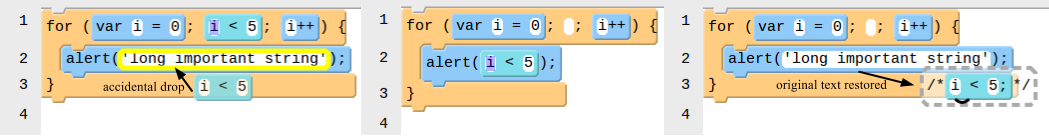
\includegraphics[width=5in]{remember-socket.png}
\caption{An Example of Droplet Restoring Old Socket Values}
\label{remember-socket}
\end{figure*}

Droplet now also remembers the old values of a socket when a block is dropped into it, so that when the block is dragged back out the socket is repopulated with the old value (fig. \ref{remember-socket}). This provides an alternate way for students to correct an accidental drop by moving the block to its intended location.

Because Droplet frequently reparses blocks, attaching the remembered value data directly to the socket is not possible. Instead, Droplet maintains a map from socket locations to remembered values. By preserving the location of the socket (using the same infrastructure as the new undo stack), the Droplet editor can track the socket and preserve the remembered value this until the block is deleted. The map from sockets to remembered values is also tracked in the undo stack, so the remembered values are preserved across undo and redo.

\section{Error Prevention and Recovery}

\subsection{Breakpoints and Line Annotations}

Applab had existing support for live errors and warnings and debugging breakpoints in text mode. Because Droplet blocks have a one-to-one relationship with text code, adding breakpoint and live line-annotation support to Droplet could easily take advantage of Applab's existing debugging infrastructure. Line breakpoints and live annotations are a part of most major professional development environments, including Applab's text mode and Eclipse \cite{Eclipse}. A study by Murphy \cite{Murphy} found that over 70\% of Eclipse users use breakpoints. In 1986 Baecker \cite{Baecker} proposed "Metatext" or annotations as one of the five main principles of program visualization.

This is a unique opportunity for Droplet, because it has a one-to-one relationship to text code. Neither Scratch nor Blockly have support for line annotations or line breakpoints.

\begin{figure}
\centering
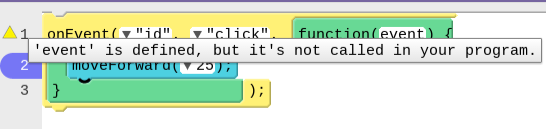
\includegraphics[width=2.5in]{breakpoint_annotations.png}
\caption{An Example of Droplet Gutter Decorations in Applab}
\label{breakpoints}
\end{figure}

Droplet now supports breakpoints and annotations in the gutter the same way major text editors do (fig. \ref{breakpoints}). Droplet mimics Ace editor's API to allow Applab and other embedders to easily convert their existing debugging infrastructure from Ace editor to Droplet.

\subsection{Handling Syntax Errors}

\begin{figure}
\centering
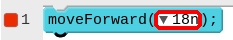
\includegraphics[width=2.5in]{error-outline.png}
\caption{Droplet's New Behavior on Syntax Errors}
\label{error}
\end{figure}

Droplet allows users to type free-form text into sockets, which it will reparse on-the-fly and turn into blocks. This helps give students the experience of writing text without switching fully to text mode. However, it also means that users can create syntax errors by typing into sockets, unlike in other major block languages. Scratch and Blockly will only allow valid inputs in text areas. Droplet will now outline the violating input when a syntax error is created, and supports error annotations to help users identify the error (fig. \ref{error}).

\section{Recognition Rather than Recall: Dropdowns in a Text-Based Editor}

Because all Droplet blocks are generated from text, Droplet did not have good support for dropdowns from sockets, which other major block languages do. Dropdowns, like autocomplete in text code, help students remember what parameters are valid, in accordinance with Neilsen's heuristic of recognition vs. recall \cite{Neilsen}.

Both Scratch and Blockly implement dropdowns for their text inputs. Both have special selectors for colors, allowing users to use a color picker or to "eyedrop" existing pixels on the screen.

\begin{figure}
\centering
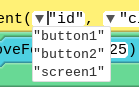
\includegraphics[width=1.5in]{dropdowns.png}
\caption{An Example of Droplet Dropdowns in Applab}
\label{dropdowns}
\end{figure}

Droplet added new configuration to allow the embedding application layer to specify dropdowns. Embedders may specify dropdowns by function name and argument position in JavaScript and CoffeeScript mode -- for instance, in Figure \ref{dropdowns}, the "fd" function has a dropdown specified at argument 0. Dropdowns can be dynamically generated -- in Figure \ref{dropdowns}, a list of element ids is generated using information taken from Applab's WYSIWYG HTML Design Mode.

\begin{thebibliography}{1}

\bibitem{Droplet}
  Bau, D. A. Droplet, A Blocks-Based Editor for Text Code. Journal of Computer Science in Colleges. 30, 6 (June 2015).
\bibitem{Code.org}
  Code.org. http://code.org
\bibitem{Eclipse}
  Mars Eclipse. http://eclipse.org
\bibitem{Weintrop}
  Weintrop, D. and Wilensky, U. To Block or Not To Block, That is the Question: Students' Perceptions of Block-based Programming. IDC '15 proceedings (June 2015).
\bibitem{Baecker}
  Baecker, R. and Marcus, A. Design Principles for the Enhanced Presentation of Computer Program Source Text. CHI '86 proceedings (April 1986).
\bibitem{Murphy}
  Murphy, G. Kersten, M. and Findlater, L. How Are Java Software Developers Using the Eclipse IDE? IEEE Software (July/August 2006) 72-82.
\bibitem{Neilsen}
  Nielsen, J. (1994). Heuristic evaluation. In Nielsen, J., and Mack, R.L. (Eds.), Usability Inspection Methods, John Wiley \& Sons, New York, NY
\bibitem{Scratch}
  Scratch. https://scratch.mit.edu/
\bibitem{Blockly}
  Blockly. https://blockly-games.appspot.com/
\bibitem{Maloney}
  Maloney, J., Resnick, M., Rusk, N., Silverman, B., and Eastmond, E. 2010. The scratch programming language and environment. ACM Trans. Comput. Educ. 10, 4, Article 16 (November 2010), 15 pages. DOI = 10.1145/1868358.1868363. http://doi.acm.org/10.1145/1868358.1868363.

\end{thebibliography}

% that's all folks
\end{document}


